\section{Les CNN}

\fancyhead[R]{\textit{\nouppercase{\leftmark}}}

\subsection{Le modèle du CNN}

Bien qu'étant un modèle efficace, le perceptron reste cependant coûteux en calcul : il faut réaliser les opérations matricielles sur tous les neurones de chaque couche.
Les réseaux neuronaux convolutifs (convolutional neural network (CNN) en anglais) permettent de réduire le nombre de calculs réalisés. Ils se basent sur la structure de données à classifier.
Les images sont un bon exemple de structure permettant de diminuer le nombre de calculs à réaliser. En effet, une image peut être caractérisée par les motifs locaux qui la constituent. Ces motifs sont en général localisés. Il n'est donc pas nécessaire de chercher un lien entre deux points éloignés d'une image.

Les CNN (Convolutionnal Neural Networks) sont entraînés à chercher des motifs sur une partie restreinte de l'image.
Le principe est le même que celui des perceptrons, sauf qu'au lieu d'appliquer un réseau entièrement connectés sur toutes les couches, on va réaliser une convolution par différents filtres sur l'image. Chaque filtre aura pour but de détecter un motif dans l'image.

Une couche d'un CNN est typiquement constituée de 3 éléments : 

1) Une couche de convolution

2) Une couche d'activation 

3) Une couche de pooling


La couche de convolution prend en entrée une image de dimension (H, L, N) avec H la hauteur de l'image, L sa largeur et N le nombre de channels (pour une image RGB, on aura N = 3). 
On applique en parallèle sur cette images M filtres de dimension identique (h, l, n) avec n = N.
La sortie de chaque filtre correspondra à un des M channels de l'image de sortie.

\begin{figure}[h]
 \centering
 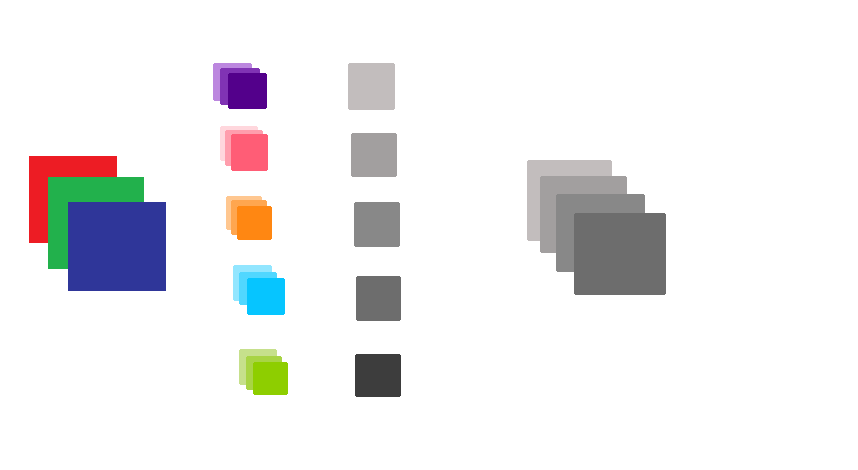
\includegraphics[width=0.7\textwidth]{img/CNN_filtres.png}
 \caption{Principe des filtres de convolution}
\end{figure}

Pour une image I de dimension (H, L, N) et un filtre F de dimension (h, l, N), on obtient une image J de dimension (H-h, L-l), la convolution est réalisée de la manière suivante :

\begin{equation}
    J(x, y) = I \star H (x, y) = \sum_{i=0}^{h - 1} \sum_{j=0}^{l- 1} \sum_{k=0}^{N - 1} I(x+i, y+j, k) \times H(i, j, k)
\end{equation}

On obtient alors une sortie de dimension (H-h, L-l, M).

Intuitivement, cette partie sert à chercher la ressemblance entre le filtre et l'image.
On devrait avoir J(x,y) < 0 si la partie de l'image I en (x,y) est très différente du filtre appliqué, et J(x,y) > 0 sinon, avec un score plus ou moins élevé selon la ressemblance.


On applique ensuite la couche d'activation. On utilise une fonction non-linéaire comme dans le cas du perceptron. 
Généralement, la fonction utilisée pour les couches de convolution intermédiaires est la fonction reLU :

\begin{equation}
    reLU (x) = x
\end{equation} si x > 0
\begin{equation}
    reLU (x) = 0 
\end{equation} sinon


\newpage 

Cette partie sert à ramener le résultat dans les réels positifs pour éviter une divergence au niveau des calculs, et pour augmenter l'écart relatif entre un bon score et un mauvais score : un score de 0 et en score de -1 obtenu lors de la convolution sont alors considéré comme tout aussi mauvais.

Enfin, on applique une couche de pooling, qui sert à réduire le nombre de données obtenues en sortie des 2 couches précédentes.
Le pooling cherche à "résumer" les scores d'une partie de l'image, en donnant un score qui dépend des pixels de cette partie.
Il existe plusieurs méthode de pooling, comme par exemple le pooling par moyenne, ou le pooling par maximum, qui est plus utilisé en pratique :
pour une image J, on choisi un paramètre S (S < L, H), et on otient la sortie K telle que :

\begin{equation}
    K(x, y) = max_{i,j \in [0, S-1] ^2 } { J(x \times S + i , y \times S + j ) }
\end{equation}


On peut ainsi enchainer les couches de convolution jusqu'à une couche finale, qui sera ensuite reliée à un réseau complètement connecté (qui n'est rien d'autre qu'un simple perceptron), pour pouvoir exploiter les résultats obtenus jusque là.
Les poids à optimiser sont alors les poids des matrices "filtres", et les poids de la couche entièrement connectée.
Dans le principe, un CNN est comme un perceptron (à part pour la couche de pooling, on pourrait construire un CNN avec un perceptron), à l'exception que certains poids sont liés lors de l'apprentissage. 

\subsection{Application pratique}

Afin de mieux comprendre le principe du CNN, nous avons réalisé un exemple simple mais clair : 
\begin{figure}[h]
 \centering
% \includegraphics[width=0.7\textwidth]{img/cnn_exemple/}
 \caption{Image à reconnaître}
\end{figure}


\newpage

\subsection{Utilisation de TensorFlow}

TensorFlow a été utilisé pour coder le CNN. Un codage à la main du CNN aurait été possible et très instructive mais complexe et chronophage. L'utilisation de TensorFlow a permis d'avancer plus rapidement sur la programmation du CNN. Par ailleurs, le fonctionnement de chaque bloc utilisé par TensorFlow pour coder un CNN avait été vu en détail précédemment, ce qui a permis de comprendre ce qui se cachait derrière les fonctions de haut niveau proposées par TensorFlow.

TensorFlow est facile d'installation sous Linux et sa prise en main est plutôt aisée. Il existe de nombreux tutoriels pour construire des CNN. Cependant, le développement de TensorFlow évolue rapidement et la documentation n'est pas forcément très complète. L'implémentation de fonctionnalités précises est donc parfois difficile. Il est nécessaire de faire de longues recherches pour trouver les fonctions désirées.

Cependant, en plus de réduire grandement le temps nécessaire pour programmer un CNN efficace, TensorFlow offre une interface graphique très utile pour suivre en direct la convergence du CNN. On peut ainsi détecter rapidement le mauvais paramétrage de notre CNN et le modifier sans attendre d'avoir mis à jour notre CNN sur les $n$ batches prévus à l'avance.

%\begin{figure}[h]
% \centering
% 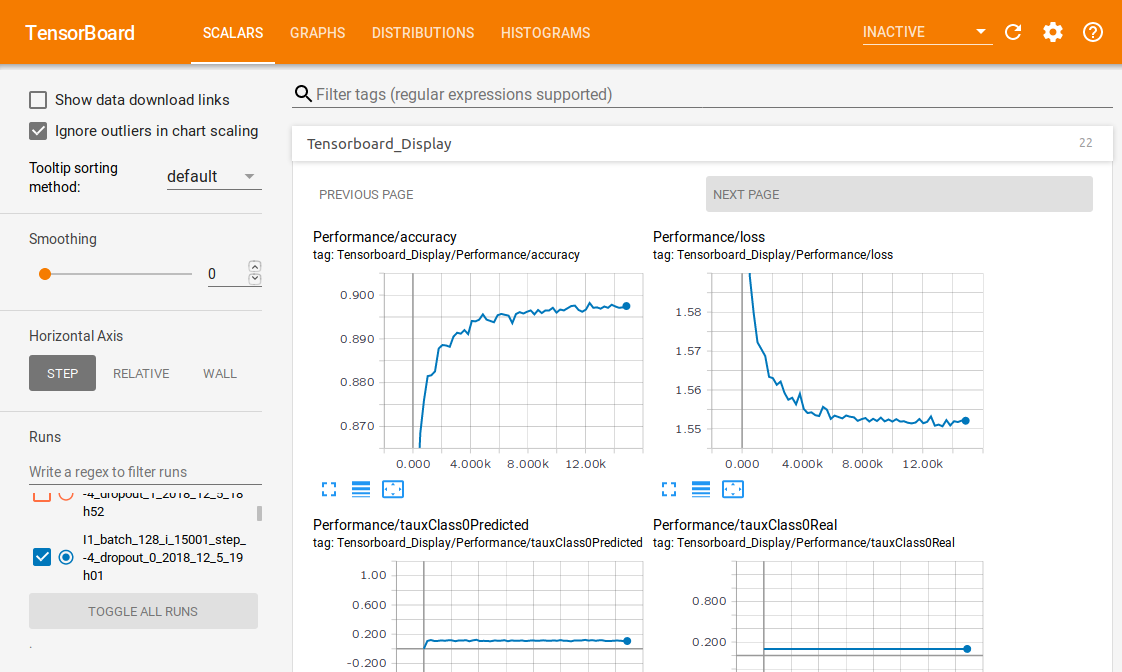
\includegraphics[width=0.7\textwidth]{img/interface_TF.png}
% \caption{Image à reconnaître}
%\end{figure}

L'exploitation des résultats a posteriori s'est avérée plus compliquée. L'interface de TensorFlow offrant des fonctionnalités plutôt limitées, l'utilisation d'un post-traitement s'est avéré indispensable. Il est par exemple impossible de réaliser des moyennes sur plusieurs runs. Après quelques recherches, nous avons réussi a extraire le taux de réussite en fonction du nombre d'apprentissages à partir des données brutes générées par TensorFlow. L'extraction du taux de réussite en fonction du temps de calcul s'est avéré plus compliquée. Nous remercions Julien \textsc{Gérard} qui nous a beaucoup aidé sur ce point. Il nous a en effet indiqué avoir trouvé dans le code source de TensorFlow la fonction $wall\_time$ qui permet d'extraire le temps écoulé depuis le lancement des calculs pour chaque relevé du taux de réussite.

Le post-traitement nous a permis de travailler sur l'évolution du taux de réussite en fonction du nombre d'apprentissage et en fonction du temps.